\begin{multicols}{2}
	\begin{center}
	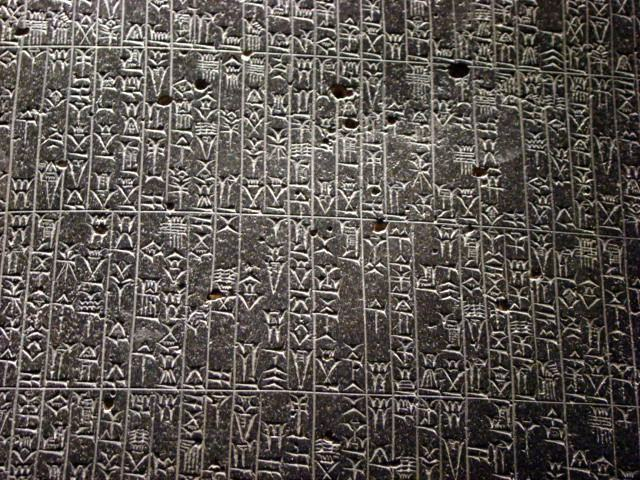
\includegraphics[width=\linewidth]{./IMG/codigo-de-hamurabi.jpg}
\end{center}	
	\vfill
	\columnbreak
	
	\begin{center}
		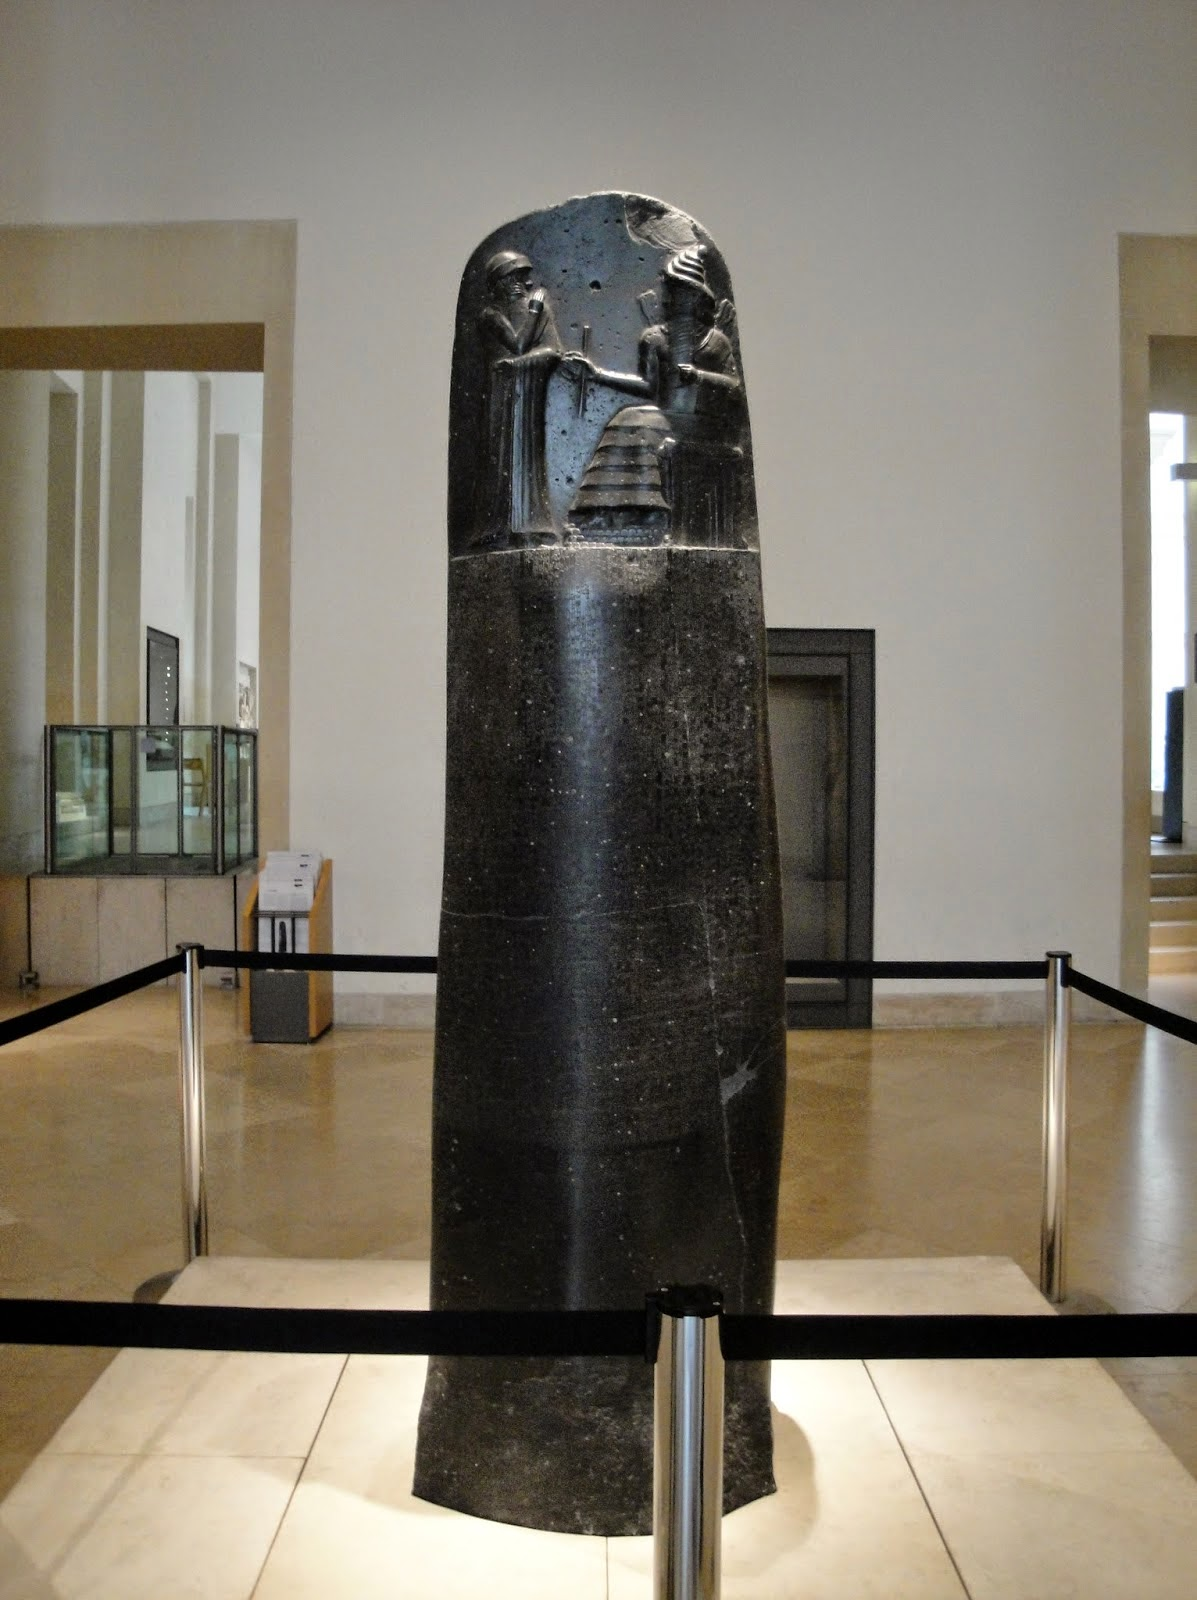
\includegraphics[height=.8\textheight]{./IMG/codigo de hamurabi.JPG}
	\end{center}

	\vfill
\columnbreak

{\Large $\sim$1754 A.C.}

{\large

\begin{itemize}
	\item Lei de Talião (olho por olho, dente por dente):

{\normalsize \subitem Punição proporcional ao crime.}

\item Responsabilidade individual:

{\normalsize \subitem Pune tanto o culpado quanto sua família se estiverem envolvidos no crime.}

\item Presunção de inocência:

{\normalsize \subitem Quem acusa deve provar.}

\item Leis relacionadas à propriedade:

{\normalsize \subitem Contratos, transações comerciais e propriedade, penas para roubo e falsificação.}

\item Questões familiares:

{\normalsize \subitem Questões familiares, como casamento, divórcio e herança.}

\item Leis de comércio:

{\normalsize \subitem Regulamentos para atividades comerciais, estabelecendo padrões e punições para práticas desonestas.}

\item Leis trabalhistas:

{\normalsize \subitem Relações de trabalho, salários e penalidades para trabalhadores que não cumpram seus deveres.}

\item Leis religiosas:

{\normalsize \subitem Práticas religiosas e rituais, indicando a influência da religião na sociedade e na legislação.}

\end{itemize}}

\vfill
\columnbreak

\large

\begin{itemize}
	
	\item \textbf{Lei 196:}
		\subitem Se um homem destruir o olho de outro homem, então seu próprio olho será destruído.
	
	\item \textbf{Lei 200:}
		\subitem Se um homem arrancar o dente de outro homem, então seu próprio dente será arrancado.
		
		\vfill\null
		\columnbreak

	\item \textbf{Lei 229:}
		\subitem Se um construtor construir uma casa para alguém, mas não a fizer de forma sólida e a casa desabar, então o construtor será morto.
	
	\item \textbf{Lei 108:}
		\subitem Se um homem acusar outro homem de assassinato, mas não puder prová-lo, então aquele que fez a acusação será morto.

	
	\item \textbf{Lei 196:}
		\subitem Se um homem em um julgamento subornar testemunhas ou juízes, então ele será morto.

\end{itemize}

\end{multicols}

\vfill
\pagebreak

